\section{Precision-Performance Optimizations}
\label{sec:precision}

\subsection{A new version of multi-grid algorithm}

\leo{Observing the initial results presented on Figure~\ref{fig.first_tests},
one can notice that independently of how many relaxations are performed, or
which cycle shape is used, and more importantly, of how many cycles are
executed, the residual norm of the algorithm reaches a lower bound (it is
around $10^{-15}$).} This bound comes from the internal limitations of the
\texttt{double} floating-point representation.  Indeed, a double uses 8 bytes
(52 bits for the mantissa, 11 for the exponent and 1 bit for the sign).
Naturally, a space-constrained representation does not allow a full description
of all rational numbers (for example between $2^{52}$ and $2^{53}$ only
integers can be represented).  If we increase the number of bits used in the
representation we can describe more and more numbers. Similarly, if we reduce
the number of bits used in the representation, we lose accuracy for numbers
that are not fully representable.

The advantage of using lower precision for the floating point operations is a
faster and more energy-efficient computation. \leo{The reason for these gains
is that floating-point units (FPUs) require more circuit logic (silicon for
ASICs, LABs/DSPs for FPGAs) for high precision operators. Thus, reducing
precision allows more low precision FPUs, which increases the Instruction-Level
Parallelism (ILP) or Vectorization that the processor can reach, hence
increasing its peak performance.}

\leo{Considering our algorithm, lower precision computations could be used if
the required accuracy allows it. For instance, if the final result should have
an accuracy} of only $10^{-3}$ then the 64 bits \texttt{double} floating-point
representation is not needed to reach it, a lower precision is enough.
Moreover, analysing the presented results, it seems clear than during the first
cycles the accuracy is low and it does not require the full precision offered by
the double floating-point representation. This observation opens to door for
making use of lower precisions temporarily during the first cycles. Therefore, it
is important to study the impact of precision on performance for MG algorithms.

\leo{To study the trade-off between precision and performance,} we modify the
relaxations step of the algorithm (remind that it is the more time consuming
part of the algorithm). In this function we can find 13 internal variables that
are originally of type \texttt{double}: 5 arrays and 8 scalars. We then propose
the following two modified versions of the MG algorithm.

\begin{itemize}

    \item \textbf{AMGfloat}, which changes the type of the 13 variables from
        \texttt{double*} or \texttt{double} to \texttt{float*} or
        \texttt{float}.

    \item \textbf{AMGmpfr(b)}, which makes use of the library
        MPFR~\cite{MPFR,MPFR_link} that introduces a type \texttt{mpfr\_t}.
        This type has a parameter $b$ which is the number of bits used in the
        mantissa of the variable. Every computation is done first in full
        precision and then rounded to a number with a mantissa using the number
        of bits given as parameter. In this version of the algorithm \emph{AMG}
        the 8 scalar variables of the relaxation function are replaced by
        \texttt{mpfr\_t} variables, all using the same number of $b$ bits for
        the mantissa.

\end{itemize}

Finally, we will denote by \emph{AMG} this original algorithm.  In terms of
arithmetic precision, \emph{AMG} behaves similarly to \emph{AMGmpfr(53)} and
\emph{AMGfloat} to \emph{AMGmpfr(24)}. There can be small differences depending
on the rounding method used.

Figure~\ref{fig.bits_accuracy} shows the accuracy that can be reached with
\emph{AMGmpfr(8)}, \emph{AMGmpfr(16)}, \emph{AMGfloat}, \emph{AMGmpfr(32)} or
\emph{AMGmpfr(64)}. The problem used is \textsc{Unstructured-Anisotropy}, with
2x2x2 processor topology and 20x20x20 matrix size. What we actually see on this
figure is the lower bound reached depending on the number of bits used.
However, before reaching this lower bound, all precisions show the same
accuracy. This means that, for example, while the accuracy of the solution is
below the threshold using single precision (32 bits), using 32 or a greater
precision to do the same computations will result in the same accuracy.
However, we expect single precision computations to be more efficient than
higher precisions in terms of time, space and energy.

\begin{figure}[htb]
    \centering
    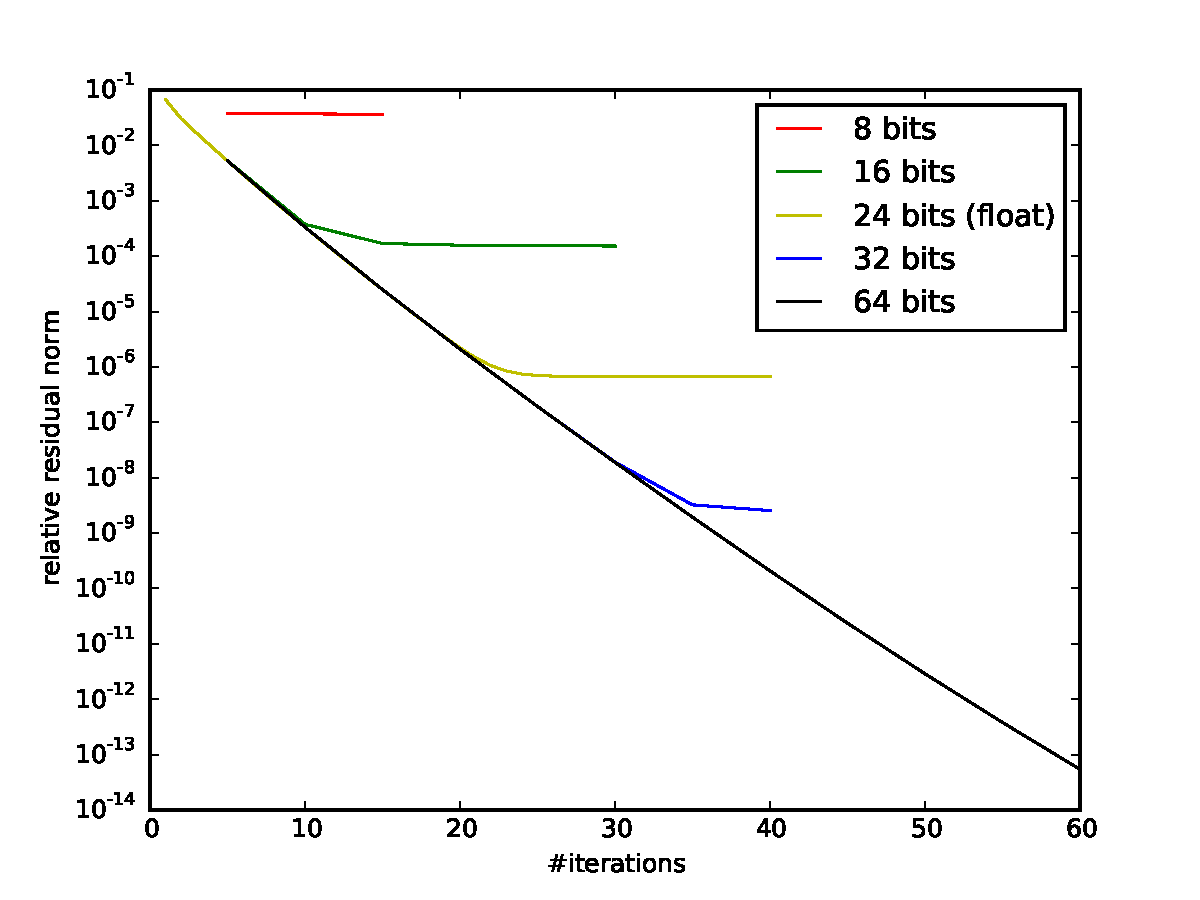
\includegraphics[width=0.9\linewidth]{figs/bits_convergence.pdf}
    \caption{Accuracy for different number of mantissa bits.}
%    Points (except for 24 bits) were obtained only for multiples of 5
%    iterations, but it is enough to see the thresholds appear.}
    \label{fig.bits_accuracy}
\end{figure}

The second thing we observe is that \emph{AMGfloat} \ldo{You use different
labels in the legend} behaves exactly as what we would expect from
\emph{AMGmpfr(24)} in terms of accuracy: it shows the same accuracy as versions
with more precision in the beginning, then it reaches a threshold between that
of \emph{AMGmpfr(16)} and that of \emph{AMGmpfr(32)}. \leo{It is important to
notice that in the \emph{AMGfloat} version more variables were changed from
\texttt{double} to \texttt{float}, however in the \emph{AMGmpfr(24)} version we
do not observe more accuracy degradation. This is because only} a few
variables from the 8 scalars control the final precision as they are temporary
variables used for intermediate computations before being plugged back into the
input matrix/vector.

Given this analysis, we design a new algorithm that adapts the precision of the
variables during the execution. It is the same algorithm as \emph{AMGmpfr(b)}
except this time the precision can change between two cycles.  We fix a
threshold on the ratio between the relative residual norm of two consecutive
steps to trigger the precision change if the gradient is lower than the
threshold (i.e., limited gain in accuracy between two consecutive cycles). Then,
we define the following 3 strategies.

\begin{itemize}

    \item start at $b=16$ and do $b=b+8$ on threshold

    \item start at $b=32$ and do $b=b+8$ on threshold

    \item start at $b=16$ and do $b=b\times2$ on threshold

\end{itemize}

We run these strategies on a 240x240x240 matrix size with a 3x3x3 topology for
\textsc{3DLaplace-27pt}. Figure~\ref{fig.prec_incr} presents the evolution of
accuracy for the original algorithm and the 3 new adaptive strategies
introduced.  We see some steps appear, corresponding to the lower bound on the
accuracy at the current precision. Then, the precision is adapted to be able to
improve the overall accuracy. Even if we lose some accuracy when waiting for
the ratio between two consecutive relative residual norm to reach the
threshold; when the precision changes the convergence rate is more important
(for one cycle) than that of the original double-precision algorithm (i.e. the
slope is bigger), allowing the adaptive strategies to quickly \emph{catch-up}
any accuracy loss and reach the maximum accuracy (of $4.7\times 10^{-13}$) in
the same number of cycles as the original full precision algorithm (20-21
cycles).

\begin{figure}[htb]
    \centering
    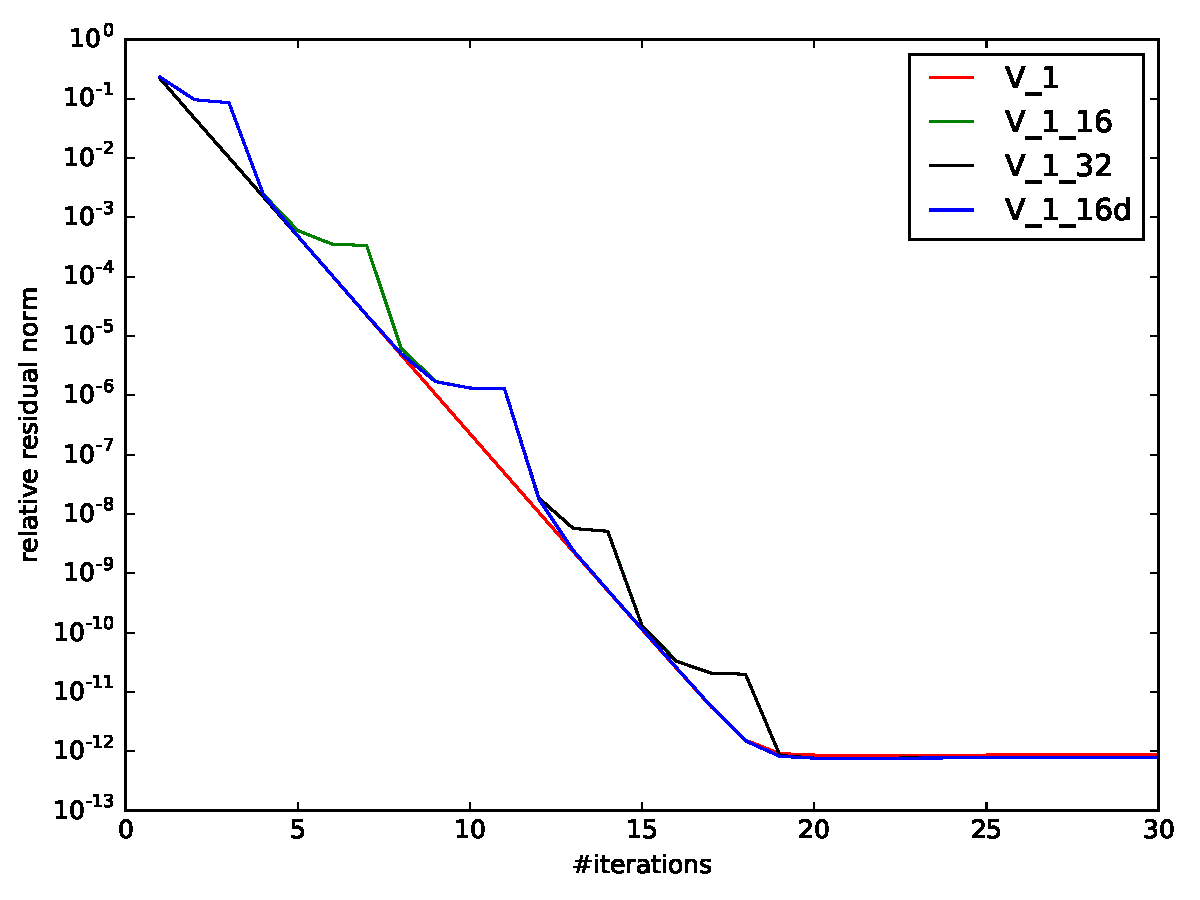
\includegraphics[width=0.9\linewidth]{figs/prec_incr.pdf}
    \caption{Accuracy of adaptive algorithms compared to the original
    double-precision with a precision threshold of $0.8$.}
    \label{fig.prec_incr}
\end{figure}

\leo{These results demonstrate that adaptive precision can be used to reach the
same accuracy in the same number of cycles, while each cycle is expected to be
less energy and time consuming because of lower precision.} At this point two
questions arise. How to evaluate the energy/time savings of this adaptive
algorithm in a hypothetical hardware with multiple precisions available? Which
precisions should be used to maximize these savings? The complexity to answer
these questions comes from the fact that the MPFR library used to do these
accuracy experiments introduces a huge overhead in the computation. For
instance, running \emph{AMGmpfr(53)} is about 20 times more time consuming than
running the classic \emph{AMG}, whereas it represents the same double-precision
algorithm.  Moreover, this overhead is not influenced by the choice of the
number of bits.  \leo{Therefore, we cannot use the execution times of the
computations done with MPFR as representatives of performance differences at
different precisions.}



